%!TEX root = ../main.tex

\chapter*{Dataframe (exam 7/7/17 - exercise 13)}
\thispagestyle{empty}

A \texttt{DataFrame} is a 2-dimensional labeled data structure with columns of the same type. You
can think of it like a spreadsheet or a table. The nice property of a \texttt{DataFrame} is that you
can access its columns by name and apply to every column functions like mean, max, etc. 

Figure \ref{dataF1} shows, as an example, a \texttt{DataFrame} including two columns storing temperatures and humidity for a weather forecast application.

You have to provide the definition of the \texttt{DataFrame} class, storing elements of type \texttt{double} and optime your choice for the \textbf{worst case complexity} under the assumption your data structure have a very large number of columns. You can assume that the columns are dense. In particular, you have to:
\begin{enumerate}
\item Provide the declaration of the \texttt{DataFrame} internal data structure.
\end{enumerate}

and you have to provide the implementation of the following methods:

\begin{enumerate}
\setcounter{enumi}{1}

\item A constructor that receives one single string as parameter. Using spaces as word
separators, it will initialize the column names with the words contained in the argument.
For example, the \texttt{DataFrame} in Figure \ref{dataF1} can be obtained passing "temperatures
humidity".

For the constructor implementation you can rely on the
\begin{equation*}
    \texttt{vector<string> split(const string \& s, char d)}
\end{equation*}
function, which returns the names of columns in \texttt{s} separated by the delimiter \texttt{d}. In other words, you are not required to implement \texttt{split()} yourselves.

\begin{figure}[h]
\begin{center}
  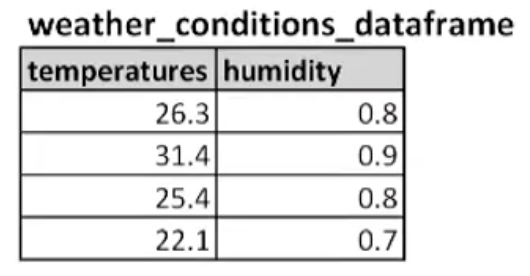
\includegraphics[width=6cm]{dataF1}
\end{center}
\caption{A weather application \texttt{DataFrame}.}
\label{dataF1}
\end{figure}

\item A \texttt{set\_column} method that, given a vector of values of type \texttt{double} and a column name, replaces the entire column content.

In order to complete this task it is better to rely on the following functions:
\begin{itemize}
    \item \texttt{check\_column\_name} checks if a given string is a existing column name in the \texttt{DataFrame};

    \item \texttt{set\_column\_data} stores, given the column name and the column data (i.e., a vector of \texttt{double}), the data in the column.
\end{itemize}

\item A \texttt{get\_column\_names} method, which returns in a \textbf{set} of \texttt{strings} the column names.

\item A \texttt{unique} method, which return the unique values (i.e., without duplicates) stored in the column whose name is passed as parameter.

\item A \texttt{drop\_column} method, which removes from the \texttt{DataFrame} the column whose name is passed as parameters.

\item A \texttt{set\_element\_at} method that, given a column name, an index \texttt{i}, and a value of type \texttt{double}, updates the i-th value of the column.

Try also to implement \texttt{get\_column} and \texttt{get\_element\_at} methods.

\item A \texttt{get\_mean} method, which returns the mean of a given column.

\item A \texttt{sum\_by\_rows} method, which returns in a vector of \texttt{double} the sum of values in each individual row of the \texttt{DataFrame}.

\item A \texttt{select\_equal} method that, given a column name and a value, returns a new \texttt{DataFrame} including only the set of rows for which the column equals the value. For instance,
\texttt{select\_equal ("temperatures", 31.4)} called on the \texttt{DataFrame} in Figure \ref{dataF1} would yield a new one with both columns, but only the second row.

\item A \texttt{concatenate} method, which returns as a copy a \texttt{DataFrame} obtained by concatenating the Dataframe with a second \texttt{DataFrame} passed as parameter (both original \texttt{DataFrame} are left unchanged). An example of concatenation is shown in Figure \ref{dataF2}.
\end{enumerate}

\begin{figure}[h]
\begin{center}
  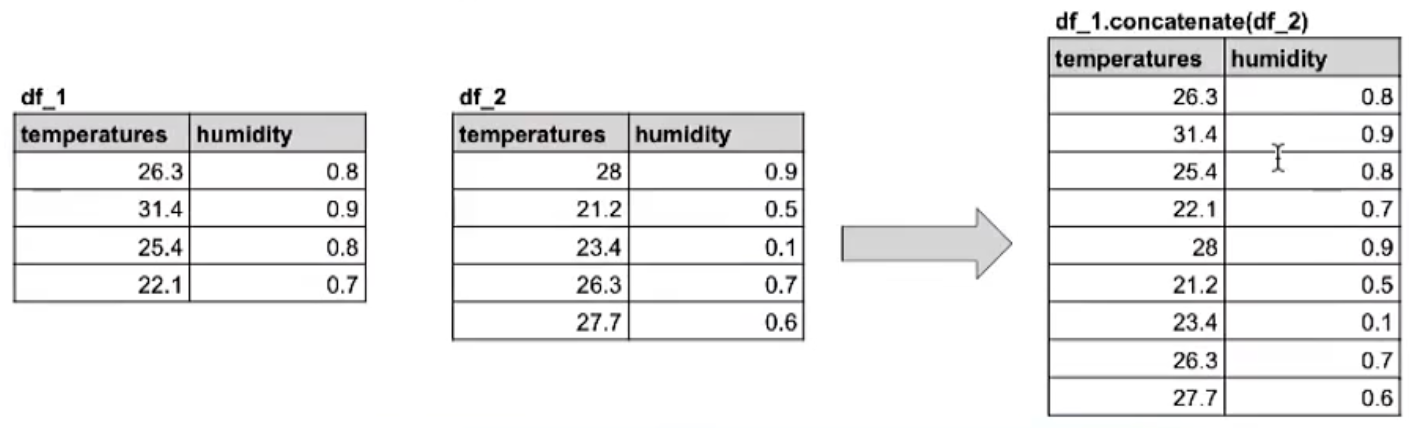
\includegraphics[width=14cm]{dataF2}
\end{center}
\caption{A concatenation of \texttt{DataFrame}s example.}
\label{dataF2}
\end{figure}

Take particular care to error conditions, for example:
\begin{itemize}
    \item access to a wrong column or element index out of range;
    \item check that all the columns have the same number of rows (which will be known only when creating the first column)
\end{itemize}

Finally,
\begin{enumerate}
\setcounter{enumi}{11}
\item Discuss the worst case complexity of the setter methods.
\end{enumerate}

